\section{Introduction}
Classic model checking algorithms often use SAT-solvers: the problem of checking of program correctness can be converted to
the instance of SAT problem, that describes an intersection of program executions language with regular language of ``bad''
executions.
In single-tread case it is known that the language of program is contained in context-free class, but in interleaved execution
scenario things become more complicated. There are a number of papers that describe 
concurrent programs behavior via Push Down Systems with synchronization actions, but our interest is around a 
\textit{shuffle} of Context-Free languages(CFL). This languages describe the interleaving of CFL
and look perfect to describe the interleaved behavior of concurrent programs.

To explain it we introduce the notion of \textit{shuffle} operation ($\odot$), that can be defined for lines as follows:
\begin{itemize}
	\item $\varepsilon \odot u = u \odot \varepsilon = {u}$, for every line $ u \in \Sigma^*$;
	\item $\alpha_1 u_1 \odot \alpha_2 u_2 = \{\alpha_1 w | w \in (u_1 \odot \alpha_2 u_2) \} \cup \newline
	\{\alpha_2 w | w \in (\alpha_1 u1 \odot u_2 ) \},  \forall \alpha_1, \alpha_2 \in \Sigma$ and $\forall u_1, u_2 \in \Sigma^*$.
\end{itemize}
Shuffle extends to languages as $L_1 \odot L_2 = \bigcup\limits_{u_1\in L_1, u_2\in L_2} u_1 \odot u_2$.

For example, $"ab" \odot "123" = \{a123b,a1b23, 12ab3, 123ab, etc.\}$.

In paper~\cite{stenman2011approximating} authors describe an approach to model checking with use of shuffle: 
context-free grammars of concurrent functions are used. 
But it is known that the shuffle of context-free languages does not contained in class of CFL and the problem of
defining either string is in the shuffle of CFL is NP-Complete. That is why an authors use a context-free approximation of 
shuffle of CFL and intersect it with error traces, but since the approximation was used this approach
didn't found some of known bugs. 
In this paper we present same approach, but without use of approximation. Instead, we narrow the context-free languages
to be shuffled and deal with NP-Completeness with SAT-Solver.


%In this work we describe an algorithm that uses shuffle of context-free languages without approximation.
%Structure will be as follows: (TODO:NOPE ) first, we propose a compact translation of CFSG into SAT.
%Second, we reduce the SAT search space by decreasing the size of languages to be shuffled.
%And third, we show how to use this technique in model checking of concurrent programs.

\section{Languages Shuffle}


Assume functions $f_1, f_2 ... f_n$ that run concurrently and context-free languages $ L_{f_1}, L_{f_2} ... L_{f_n}$
generated for each of them. We want to check a correctness of the functions execution. For that
we generate regular language $R_1$ that describes all ``bad'' executions. For example, if it is needed
to check reachability of an \textit{error} operator in program then presented in picture~\ref{ErrorStarAutomaton} automaton 
produce the desired language.
Now our task is to inspect an intersection $ (L_{f_1} \odot L_{f_2} \odot... \odot L_{f_n})\cap R_1$ --- its
emptiness means the program can not reach the \textit{error} state (we note that some conditions preserving the semantics of program
should be added to $R_1$, see the Example section).
Since generated languages (both CF and Reg) can potentially generate an infinite number of strings, then representation 
of this problem in the form of a finite SAT formula is impossible. Therefore, we narrow them to finite.
\begin{figure}[ht]
	\centering
	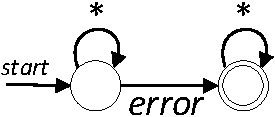
\includegraphics[scale=.6]{pic/ErrorStarAutomaton.pdf}
	\caption{Finite automaton of error traces.}
	\label{ErrorStarAutomaton}
\end{figure}



%Так как языки потенциально могут порождать бесконечное множество строк, то представить эту задачу ввиде конечной SAT
%формулы невозможно. Поэтому мы сузим язык шаффла и регулярный ддо конечных множеств.

First, we set a restriction on the length of loops in the regular language $ R_1 $. This is possible in assumption
that the error can usually be detected in the first iterations of the loops. This assumption is used in bounded model
checking~\cite{BMC}.%, but here we use the bound on traces language instead of program language.
The result of such bounding 
is regular language described by finite automaton $R_2$ without loops that produce finite set of lines.

Then we appeal to the intuition of shuffle operation. If the line $J$ is in the language $B \odot C$ then there is 
a split of $J$ of $J_B$ and $J_C$ such that $b_1 c_1 b_2 c_2 ... b_k c_k = J$ where $b_i, c_i \in (\Sigma^* \cup \varepsilon)$
and $b_1 b_2 ... b_k = J_B, c_1 c_2 ... c_k = J_C$. Both $J_B$ and $J_C$ are in the language $J'$ ---
the language of lines $J$ with all possible omissions of terminals.
For the finite automaton $R_2$ the desired language of lines with omissions is described by an automaton $R_2'$ ---  
an epsilon-closure of $ R_2 $.

Since the language of $R_2'$ is finite, we can consider the languages
$ L_{f_i}' = L_{f_i} \cap R_2', i \in 1..n$ --- the finite context-free narrowing of languages $ L_{i}$.
Thus, we redefine initial problem of language intersection to $(L_{f_1}' \odot L_{f_2}' \odot... \odot L_{f_n}')\cap R_2$.
All this languages are finite therefore we can generate a SAT problem instance to check intersection emptiness.

An instance of SAT problem is a boolean formula which is checked by solver for satisfiability. 
Constructing a formula for the problem defined above requires a more deep inspection of the languages' structure.
$R_2$ is a finite automaton that describes multiple paths from initial state to final. Transition labels of 
this paths define a language os that automaton. In terms of our problem we can consider the terminals of this language as 
a transitions of the form $i\_a\_j$, where $i$ and $j$ are states of $R_2$; $a$ --- transition label.
Since the languages $L_{f_i}'$ are $L_{f_i} \cap R_2'$, they describe the sets of transitions in 
$R_2$. Thus, the problem of giving the line from the language defined by intersection $(L_{f_1}' \odot L_{f_2}' \odot... \odot L_{f_n}')\cap R_2$
is equivalent to providing a sets $W_1...W_n$ of transitions ($W_i \in L_{f_i}'$) which preserve the following conditions:
\begin{itemize}
	\item $\bigcap\limits_{i\in 1..n} W_i = \emptyset$, i.e.
	each transition of $R_2$ contained not more then in one of the sets $W_i$.
	\item $\bigcup\limits_{i\in 1..n} W_i \in R_2$, i.e. union of all transitions
	is a path in $R_2$ from initial to final state. 
\end{itemize}
Such problem interpretation intuitively define the rules of the SAT formula generation.
The formula consist of following parts, connected with conjunction.
\begin{itemize}
	\item Define the sets of transitions for each language $L_{f_i}'$ with the alternation
	 of formulas $(t_i^1 \& t_i^2 \& ...\& t_i^k)$, where $t_i^1 ... t_i^k$ are transitions of the same set.
	\item ...
	\item ...
\end{itemize}





\section{Example}
%Consider functions Add() and Dec() running concurrently. An \textit{error} operator stands the program reach unwanted state.
%The problem is to define either program can reach the \textit{error} operator. 



%To solve this problem we build Finite Automata to check for an emptiness an intersection $L_prog \cap L_exec$, where
%$L_prog$ is the language described by shuffle of grammars $G_add$ and $G_dec$; $L_exec$ is regular language described by Finite Automaton $R$.


%To preserve the semantics of program we need to add constraints on variables in R.


%then idea is to get formula that describes our intersection. 

%In general, CFG can't be represented by finite SAT formula, because CF grammars can produce infinite 
%lines, thus in model checking widely use bounding of loops and recursion with some N. On the other hand,
%the error traces can be bounded instead of grammars, thus we change our problem to 

%--- 


%Consider such example: we want to define either line $L = a12b3c$ is contained
%in language defined by grammar $S = A \odot B; A = 12 | 123 | a12 | 1a2; B = abc | b3c | 21a$. 

%Let us describe the main ideas of our approach to solve this problem.
%\begin{itemize}
%	\item Generate language $L'$ of all subsequences of $L$, e.g. $L' = \{a, a23, 123, bc, abc, ...\}$.
%	\item Find the intersections of $L'$ with languages of grammars $A$ and $B$. 
%	      The results are:
%	      \begin{itemize}
%	      		\item $L'_A = L' \cap L_A = \{12, 123, a12\}$;
%				\item $L'_B = L' \cap L_B = \{abc, b3c\}$.
%	      \end{itemize}
%    \item Find a pairs of lines $\{(l'_A, L'_B) : l'_A \in L'_A, L'_B \in L'_B\}$ that can be shuffled to get line $L$. 
%          This pairs are $(123, abc)$ and $(a12, b3c)$. thus we can say that language defined with $G_1$ contains $L$.
%\end{itemize}

%Parsing of regular languages described in~\cite{Grigorev}

\section{Conclusion}

